\section{A detailed explanation of the attributes of the data}
\subsection*{Attribute information}
	\begin{enumerate}
	\item X - x-axis spatial coordinate within the Montesinho park map: 1 to 9
	\item Y - y-axis spatial coordinate within the Montesinho park map: 2 to 9
	\item month - month of the year: "jan" to "dec" 
	\item day - day of the week: "mon" to "sun"
	\item FFMC - The Fine Fuel Moisture Code (FFMC) is a numeric rating of the moisture content of litter and other cured fine fuels. This code is an indicator of the relative ease of ignition and the flammability of fine fuel
	\item DMC - The Duff Moisture Code (DMC) is a numeric rating of the average moisture content of loosely compacted organic layers of moderate depth. This code gives an indication of fuel consumption in moderate duff layers and medium-size woody material.
	\item DC - The Drought Code (DC) is a numeric rating of the average moisture content of deep, compact organic layers. This code is a useful indicator of seasonal drought effects on forest fuels and the amount of smoldering in deep duff layers and large logs.
	\item ISI - The Initial Spread Index (ISI) is a numeric rating of the expected rate of fire spread. It combines the effects of wind and the FFMC on rate of spread without the influence of variable quantities of fuel.
	\item temperature in Celsius degrees: 2.2 to 33.30
	\item RH - relative humidity in %: 15.0 to 100
	\item wind - wind speed in km/h: 0.40 to 9.40 
	\item rain - outside rain in mm/m2 : 0.0 to 6.4 
	\item area - the burned area of the forest (in ha): 0.00 to 1090.84 
	\end{enumerate}	

\subsection*{Describe if the attributes are discrete/continous, Nominal/Ordinal/Interval/Ratio.}
	\begin{enumerate}
	\item X - Discrete, Nominal
	\item Y - Discrete, Nominal
	\item month - Discrete, Ordinal
	\item day - Discrete, Ordinal
	\item FFMC - Continous, Interval
	\item DMC - Continous, Interval
	\item DC - Continous, Interval
	\item ISI - Continous, Interval
	\item temp - Continous, Interval
	\item RH - Continous, Ratio
	\item wind - Continous, Ratio
	\item rain - Continous, Ratio
	\item area - Continous, Ratio
	\end{enumerate}
\subsection*{Give an account of whether there are data issues (i.e. missing values or corrupted data) and describe them if so.}
There is no missing values or corrupted data.
\subsection*{Describe the basic summary statistics of the attributes.}
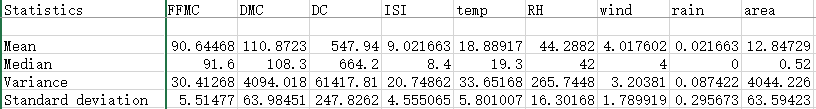
\includegraphics[width=\textwidth]{summary_statistics.png}